\chapter{Variabili aleatorie}
\section{Variabili aleatorie}
Capita spesso che studiando un fenomeno aleatorio (casuale) si sia più interessati a una qualche funzione dei possibili esiti che agli esiti stessi, queste funzioni a valori reali definite sullo spazio campionario sono note come \textit{variabili aleatorie}. Dato che il valore di una variabile aleatoria è determinato dall'esito dell'esperimento, possiamo assegnare le probabilità ai possibili valori ottenuti dalla variabile aleatoria.

\begin{Example}{}{}
    \textit{Supponiamo che il nostro esperimento consista nel lanciare 3 monete equilibrate. Se denotiamo con Y il numero di teste che si ottengono, allora Y è una variabile aleatoria che assume i valori 0, 1, 2, 3 con le seguenti probabilità:}
    \begin{align*}
        &P\{Y = 0\} = P\{(C,C,C)\}=\frac{1}{8}\\
        &P\{Y = 1\} = P\{(C, C, T), (C, T, C), (T, C, C)\} = \frac{3}{8}\\
        &P\{Y = 2\} = P\{(C,T,T),(T,C ,T),(T,T,C)\} = \frac{3}{8}\\
        &P\{Y = 3\} =P{(T,T,T)} = \frac{1}{8}
    \end{align*}
    Siccome $Y$ deve assumere uno tra i valori 0,1,2 e 3, abbiamo:
    \begin{equation*}
        1=P(\bigcup^3_{i=0}\{Y=i\})=\sum^3_{i=0}P\{Y=i\}
    \end{equation*}
\end{Example}

\begin{Example}{}{}
    \textit{Estraiamo quattro palline a caso senza reinserimento da una scatola che contiene venti palline numerate da 1 a 20. Se X denota il numero più grande tra i quattro estratti, allora X sarà una variabile aleatoria che può assumere i valori 4, 5, ..., 20. Poiché ognuna delle $\binom{20}{4}$ possibili quaterne di palline può essere ugualmente estratta, la probabilità che X assuma ognuno di questi valori è:}
    \begin{equation*}
        P\{X=i\}=\frac{\binom{i-1}{3}\binom{1}{1}}{\binom{20}{4}}\hspace{1cm}i=4,...,20
    \end{equation*}
    Questo perché il numero di quaterne che fanno sì che $X = i$ è pari al numero di selezioni di quattro palline tra le quali sia presente quella con il numero i e tre numerate da 1 a $i - 1$. Essendoci $\binom{1}{1}\binom{i-1}{3}$ possibili scelte di tali quaterne, da questo si ricava la precedente espressione.
    
    Supponiamo ora che si desideri calcolare $P\{X > 10\}$. Chiaramente un modo per farlo è utilizzare la precedente formula ottenendo:
    \begin{equation*}
        P\{X>10\}=\sum^{20}_{i=11}P\{Y=i\}=\sum^{20}_{i=11}\frac{\binom{i-1}{3}}{\binom{20}{4}}
    \end{equation*}
    Tuttavia, un approccio più diretto per determinare $P\{X > 10\}$ potrebbe essere di considerare:
    \begin{equation*}
        P\{X > 10\} = 1 - P\{X \leq 10\} = 1 - \frac{\binom{10}{4}}{\binom{20}{4}}
    \end{equation*}
\end{Example}

\begin{Definition}{Distribuzione di $X$}{}
    Data una variabile casuale $X$, definiamo distribuzione di $X$ la funzione:
    \begin{equation*}
        F(b):=P(X\leq b)\hspace{1cm}b\in(-\infty,+\infty)
    \end{equation*}
\end{Definition}

\begin{Lemma}{}{}
    $b'>b\implies F(b')\geq F(b)$
    \begin{demonstration}
        $F(b)=P(X\leq b)\leq P(X\leq b')=F(b')$. Quindi $X\leq b\implies X\leq b'$ con $b'>b$ e $\{X\leq b\}\subset\{X\leq b'\}$.
    \end{demonstration}
\end{Lemma}

\section{Variabili aleatorie discrete}
Una variabile aleatoria $X$ che possa assumere dei valori in un insieme numerabile $I=\{x_1,x_2,x_3,...\}$ è detta \textit{discreta}.

\begin{Definition}{Densità discreta}{}
    Per una variabile aleatoria discreta $X$, definiamo la densità discreta $p(a)$ di $X$ come:
    \begin{equation*}
        \forall a\in I\hspace{0,5cm}p(a):=P\{X=a\}
    \end{equation*}
\end{Definition}

Può risultare istruttivo rappresentare la densità discreta in forma grafica ponendo i valori $x_i$ in ascissa e quelli della funzione $p(x_i)$ in ordinata, vedi Figura \ref{fig:aleatorie1}.

\begin{figure}[h]
    \centering
    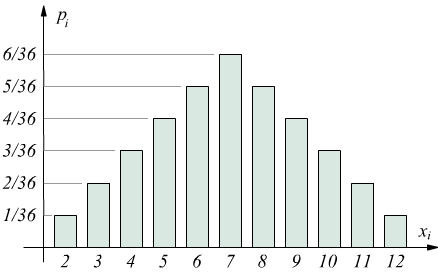
\includegraphics[width=0.5\linewidth]{images/aleatorie1.png}
    \caption{Distribuzione di probabilità nelle variabili aleatorie}
    \label{fig:aleatorie1}
\end{figure}

\begin{Example}{}{}
    \textit{La densità discreta di una variabile aleatoria $X$ è data da $p(i) = \frac{c\lambda^i}{i!}$, $i = 0,1,2,...$, dove $\lambda$ è una costante positiva. Si calcoli (a) $P\{X = 0\}$ e (b) $P\{X > 2\}$.}

    Essendo $\sum^\infty_{i=0}p(i)=1$ abbiamo che:
    \begin{equation*}
        c\sum^\infty_{i=0}\frac{\lambda^i}{i!}=1
    \end{equation*}
    implica, essendo $e^x=\sum^\infty_{i=0}\frac{x^i}{i!}$, che
    \begin{equation*}
        ce^\lambda=1\hspace{1cm}c=e^{-\lambda}
    \end{equation*}
    Perciò
    \begin{enumerate}[label=(\alph*)]
        \item $P\{X = 0\} = e^{-\lambda}\frac{\lambda^0}{0!} = e^{-\lambda}$
        \item $P\{X > 2\} = 1 - P\{X \leq 2\} = 1 - P\{X = 0\} - P\{X = 1\} - P\{X = 2\}=\\1-e^{-\lambda}-\lambda e^{-\lambda}-\frac{\lambda^2e^{-\lambda}}{2}$
    \end{enumerate}
\end{Example}

\begin{Lemma}{}{}
    $F(b)=P(X\leq b)=P(\cup_{x\in I, x\leq b}\{X=x\})=\sum_{x\in I,x\leq b}P(X=x)=\sum_{x\in I,x\leq b}P(x)$. Quindi $F(b)=\sum_{x\in I,x\leq b}P(x)$.
\end{Lemma}

Se $X$ è una variabile aleatoria discreta che assume i valori $x_1, x_2, x_3$, , dove $x_1<x_2<x3<...$, allora la sua funzione di distribuzione $F$ è costante a tratti. Ciò significa che il valore di $F$ è costante negli intervalli $[x_{i-1},x_i)$ e poi ha un salto di ampiezza pari a $p(x_i)$ in $x_i$, vedi Figura \ref{fig:aleatorie2}.

\begin{figure}[h]
    \centering
    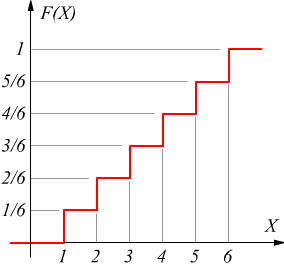
\includegraphics[width=0.3\linewidth]{images/aleatorie2.png}
    \caption{Funzione di ripartizione nelle variabili aleatorie}
    \label{fig:aleatorie2}
\end{figure}

\begin{Example}{}{}
    \textit{$X$ ha distribuzione:}
    \begin{equation*}
        F(b)=\begin{cases}
            0\hspace{1cm}b<0\\
            \frac{1}{2}\hspace{1cm}0\leq b< \frac{1}{2}\\
            \frac{3}{4}\hspace{1cm}\frac{1}{2}\leq b< 3\\
            1\hspace{1cm}b\geq 3
        \end{cases}
    \end{equation*}
    \textit{Determinare: (a) la densità discreta di $X$ e (b) $P(0\leq X\leq \frac{1}{2})$.}

    \begin{enumerate}[label=(\alph*)]
        \item $X$ ha valori in $\{0,\frac{1}{2},3\}$ con $\epsilon$ arbitrariamente piccolo si ha:
        \begin{align*}
            &P(0)=P(X=0)=F(0)-F(0-\epsilon)=\frac{1}{2}-0=\frac{1}{2}\\
            &P(\frac{1}{2})=P(X=\frac{1}{2})=F(\frac{1}{2})-F(\frac{1}{2}-\epsilon)=\frac{3}{4}-\frac{1}{2}=\frac{1}{4}\\
            &P(3)=P(X=3)=F(3)-F(3-\epsilon)=1-\frac{3}{4}=\frac{1}{4}
        \end{align*}

    \item $P(0\leq X\leq \frac{1}{2})=P(\bigcup_{i\in I:0\leq i\leq\frac{1}{2}}\{X=i\})=P(\{X=0\}\cup\{X=\frac{1}{2}\})=P(X=0)+P(X=\frac{1}{2})=\frac{1}{2}+\frac{1}{4}=\frac{3}{4}$
    
    \end{enumerate}
\end{Example}

\section{Valore atteso}
Se $X$ è una variabile aleatoria discreta con densità discreta $p(x)$, il valore atteso (o la speranza matematica) di $X$, che denoteremo con $E(X)$, è definito da:
\begin{equation*}
    E(X)=\sum_{x\in I}xp(x)=\sum_{x\in I}xP(X=x)
\end{equation*}
quindi il valore atteso di $X$ è la media pesata di tutti i possibili valori che $X$ può assumere, ognuno pesato con la probabilità che $X$ lo assuma.

\begin{Example}{}{}
    \textit{Si calcoli $E(X)$ quando $X$ rappresenta l’esito del lancio di un dado equilibrato.}
    
    Essendo $p(1) = p(2) = p(3) = p(4) = p(5) = \frac{1}{6}$ otteniamo che:
    \begin{equation*}
        E(X)=1(\frac{1}{6})+2(\frac{1}{6})+3(\frac{1}{6})+4(\frac{1}{6})+5(\frac{1}{6})+6(\frac{1}{6})=\frac{7}{2}
    \end{equation*}
\end{Example}

\begin{Example}{}{}
    \textit{Dato un evento $A$, definiamo la funzione indicatrice $I$ di $A$ come:}
    \begin{equation*}
        I=\begin{cases}
            1\hspace{1cm}\mbox{ se }A\mbox{ si verifica}\\
            0\hspace{1cm}\mbox{ se }A^c\mbox{ si verifica}
        \end{cases}
    \end{equation*}
    \textit{si calcoli $E(I)$.}

    Poiché $p(1) = P(A), p(0) = 1 - P(A)$, abbiamo che:
    \begin{equation*}
        E(I)=1P(A)+0(1-P(A))=P(A)
    \end{equation*}
    Cioè, il valore atteso della variabile indicatrice di un evento $A$ è pari alla probabilità che l'evento $A$ si verifichi. 
\end{Example}

\subsection*{Valore atteso di una funzione di una variabile aleatoria}
Supponiamo di avere una variabile aleatoria discreta $X$ e la sua densità discreta, e di voler calcolare il valore atteso di una qualche funzione di $X$, diciamo $g(X)$. Essendo $g(X)$ stessa una variabile aleatoria discreta, avrà una densità discreta, che possiamo determinare conoscendo quella della variabile $X$. Una volta determinata la densità discreta di $g(X)$ possiamo calcolare $E(g(X))$ utilizzando la definizione del valore atteso.

\begin{Example}{}{}
    \textit{Sia $X$ una variabile aleatoria che assuma i valori $-1,0,1$ con probabilità rispettivamente pari a:}
    \begin{equation*}
        P(X=-1)=0.2\hspace{1cm}P(X=0)=0.5\hspace{1cm}P(X=1)=0.3
    \end{equation*}
    \textit{si calcoli $E(X^2)$.}

    Sia $Y = X^2$, è immediato verificare che la densità discreta di $Y$ è data da:
    \begin{align*}
        &P\{Y = 1\} = P\{X = -1\} + P\{X = 1\} = 0.5\\
        &P\{Y = 0\} = P\{X = 0\} = 0.5
    \end{align*}
    Quindi:
    \begin{equation*}
        E(X^2) = E(Y) = 1(0.5) + 0(0.5) = 0.5 
    \end{equation*}
\end{Example}

\begin{Proposition}{}{}\label{prop:var-aleatoria}
    Se $X$ è una variabile aleatoria discreta, che assume i valori $x_i$ con $i\geq1$ con probabilità pari a $p(x_i)$, allora per ogni funzione a valori reali $g$:
    \begin{equation*}
        E(g(X))=\sum_{x\in I}g(x)p(x)
    \end{equation*}
    \begin{example}
        Nell'esempio precedente si può applicare questa formula per ottenere:
        \begin{equation*}
            E(X^2)=\sum_{x\in I}x^2p(x)=(-1)^20.2+(0^2)0.5+(1^2)0.3=0.5
        \end{equation*}
    \end{example}
\end{Proposition}

\begin{Corollario}{}{}\label{cor:var-aleatorie}
    Se $X$ è una variabile aleatoria discreta, e $a,b$ sono delle costanti allora:
    \begin{equation*}
        E(aX+b)=aE(X)+b
    \end{equation*}
    \begin{demonstration}
        $E(aX+b)=\sum_{x\in I}(aX+b)p(x)$, per la Proposizione \ref{prop:var-aleatoria} si ha $g(x)=aX+b$ con:
        \begin{equation*}
            a\sum_{x\in I}xp(x)+b\sum_{x\in I}p(x)=aE(X)+b
        \end{equation*}
    \end{demonstration}
\end{Corollario}

\section{Varianza}
Data una variabile aleatoria $X$ assieme alla sua funzione di distribuzione $F$, potrebbe essere estremamente utile poter riassumere le principali proprietà della funzione $F$ in termini di alcune quantità opportunamente definite. Tuttavia, sebbene $E(X)$ fornisca la media pesata di tutti i possibili valori di $X$, essa non dà alcuna informazione riguardo alla variabilità, o dispersione, di questi valori.

Per esempio date $X_1, X_2, X_3$ variabili aleatorie:
\begin{align*}
    &X_1=0\hspace{1cm}\mbox{con probabilità }1\\
    &X_2=\begin{cases}-1\hspace{1cm}\mbox{con probabilità }\frac{1}{2}\\1\hspace{1cm}\mbox{con probabilità }\frac{1}{2}\end{cases}\\
    &X_3=\begin{cases}100\hspace{1cm}\mbox{con probabilità }\frac{1}{2}\\-100\hspace{1cm}\mbox{con probabilità }\frac{1}{2}\end{cases}\\
\end{align*}

Notiamo che è presente una maggiore dispersione nei possibili valori della variabile $X_2$ piuttosto che in quelli di $X_1$ (che è addirittura costante) e nei possibili valori di $X_3$ rispetto a quelli di $X_2$. Siccome ci aspettiamo che $X$ assuma valori disposti attorno al suo valor medio $E(X)$, appare ragionevole misurare la possibile variabilità di $X$ facendo la media della distanza dal valor medio che i possibili valori della variabile X assumono.

\begin{Definition}{Varianza}{}
    Se $X$ è una variabile aleatoria di media $\mu$, allora la varianza di $X$, che denotiamo con $Var(X)$, è definita come:
    \begin{equation*}
        Var(X)=E((X-\mu)^2)=\sum_{x\in I}(x-\mu)^2p(x)
    \end{equation*}
    o alternativamente:
    \begin{equation*}
        Var(X)=E(X^2)-(E(X))^2
    \end{equation*}
\end{Definition}

Tornando all'esempio precedente abbiamo che:
\begin{align*}
    &Var(X_1)=E(X_1^2)-(E(X_1))^2=(0^2)P(X_1=0)-0=0\\
    &Var(X_2)=E(X_2^2)-(E(X_2))^2=(1)^2\frac{1}{2}+(-1)^2\frac{1}{2}-0=1\\
    &Var(X_3)=E(X_3^2)-(E(X_3))^2=(-100)^2\frac{1}{2}+(100)^2\frac{1}{2}-0=10000\\
\end{align*}

\begin{Lemma}{}{}
    Date due costanti $a$ e $b$, vale la seguente identità:
    \begin{equation*}
        Var(aX+b)=a^2Var(X)
    \end{equation*}
    \begin{demonstration}
        Per provarla, poniamo $\mu = E(X)$ e ricordiamo che per il Corollario \ref{cor:var-aleatorie} $E[aX + b] = a\mu + b$. Perciò:
        \begin{equation*}
            Var (aX + b) = E((aX + b - a\mu-b)^2) = E(a^2(X-\mu)^2) = a^2E((X-\mu)^2)=a^2Var(X)
        \end{equation*}
    \end{demonstration}
\end{Lemma}

\section{Variabili aleatorie di Bernoulli e binomiali}
Abbiamo un esperimento il cui esito è un successo o un insuccesso, ripetiamo più volte l'esperimento e vogliamo sapere la probabilità che abbia successo o insuccesso un numero di volte.

\begin{Definition}{Variabile aleatoria di Bernoulli}{}
    $X$ si dice variabile aleatoria di Bernoulli con $p\in[0,1]$ se prende valori in $\{0,1\}$ e ha densità:
    \begin{equation*}
        p(0)=1-p\hspace{1cm}p(1)=p
    \end{equation*}
    scriviamo $X\sim Bern(p)$. 
    
    \textit{Si usa una Bernoulli quando un evento si può dividere solo in successo o insuccesso.}
\end{Definition}

\begin{Definition}{Variabile aleatoria binomiale}{}
    $X$ si dice variabile aleatoria binomiale con parametri $n\in\mathbb{N}$ e $p\in[0,1]$ se ha valori in $\{0,1,...,n\}$ e densità:
    \begin{equation*}
        \forall k\in\{0,1,...,n\}\hspace{1cm}p(k)=\binom{n}{k}p^k(1-p)^{n-k}
    \end{equation*}
    scriviamo $X\sim Binom(n,p)$. 
    
    \textit{Si usa una binomiale quando si vuole conoscere il numero totale di successi ottenuti in $n$ prove indipendenti.}
\end{Definition}

Per il teorema del binomio ($(A+B)^n=\sum_{k=0}^\infty A^kB^{n-k}\binom{n}{k}$), è facile dimostrare che le probabilità della formula  del binomio dà effettivamente come somma 1; infatti:
\begin{equation*}
    \sum_{k=0}^np(k)=\sum_{k=0}^np^k(1-p)^{n-k}=(p+1-p)^n=1^n=1
\end{equation*}

\begin{Example}{Variabile aleatoria binomiale}{}
    \textit{Ogni mattina il tram fa ritardo con probabilità $\frac{1}{3}$. Qual'è la probabilità che nel mese di Novembre il tram faccia ritardo esattamente $0,3,5$ volte?}

    Indichiamo con $X$ il numero di volte che il tram fa ritardo nel mese di Novembre, vogliamo calcolare $X\sim Binom(n=30, p=\frac{1}{3})$.
    \begin{align*}
        &P(X=0)=\binom{30}{0}(\frac{1}{3})^0(\frac{2}{3})^{30}=(\frac{2}{3})^{30}\\
        &P(X=3)=\binom{30}{3}(\frac{1}{3})^3(\frac{2}{3})^{27}\\
        &P(X=5)=\binom{30}{5}(\frac{1}{3})^5(\frac{2}{3})^{25}
    \end{align*}
\end{Example}

\subsection*{Proprietà delle variabili aleatorie binomiali}
Dato $X\sim Binom(n,p)$ con $n\in\mathbb{N}$ e $p\in[0,1]$:
\begin{enumerate}
    \item $E(X)=np$
    \item $Var(X)=np(1-p)$
    \item $p(i)$ è primo strettamente crescente e poi strettamente decrescente e raggiunge il massimo nel punto:
    \begin{equation*}
        i^*=\max\{k\in\mathbb{N}_0:k\leq (n+1)p\}
    \end{equation*}
\end{enumerate}

\section{Variabile aleatoria di Poisson}
\begin{Definition}{Variabile aleatoria di Poisson}{}
    $X$ si dice variabile aleatoria di Poisson con parametro $\lambda\in(0,\infty)$ se ha valori in $\mathbb{N}_0$ e ha densità:
    \begin{equation*}
        \forall i\in\mathbb{N}_0\hspace{1cm}P(X=i)=\frac{\lambda^i}{i!}e^{-\lambda}
    \end{equation*}
    scriviamo $X\sim Poi(\lambda)$. 
    
    \textit{Si usa una Poisson quando si vuole contare il numero di successi in un dato intervallo di tempo.}
\end{Definition}

Anche questa formula definisce la densità discreta, essendo:
\begin{equation*}
    \sum^\infty_{i=0}P(X=i)=\sum^\infty_{i=0}\frac{\lambda^i}{i!}e^{-\lambda}=e^\lambda e^{-\lambda}=1
\end{equation*}

\begin{Lemma}{Variabile aleatoria di Poisson}{}
    Con $X\sim Poi(\lambda)$ abbiamo che $E(X)=\lambda$ e $Var(X)=\lambda$.
    \begin{demonstration}
        \begin{align*}
            E(X)=\sum^\infty_{i=0}ip(i)=\sum^\infty_{i=1}i\frac{\lambda^i}{i!}e^{-\lambda}=\sum^\infty_{i=1}\frac{\lambda\lambda^{i-1}}{(i-1)!}e^{-\lambda}=\lambda\sum^\infty_{i=1}\frac{\lambda^{i-1}}{(i-1)!}e^{-\lambda}=\lambda\sum^\infty_{k=0}\frac{\lambda^k}{k!}e^{-\lambda}=\lambda
        \end{align*}
    \end{demonstration}
\end{Lemma}

\begin{Proposition}{Poisson è il limite di distribuzione binomiale}{}
    Dati $X\sim Poi(\lambda)$ e $Y\sim Binom(x,p)$ abbiamo che $p_\lambda(i)=P(X=i)$ e $p_{n,p}(i)=P(Y=i)$. Consideriamo il limite $n\to\infty$ e $p=\frac{\lambda}{n}\to0$ dove $\lambda\in\mathbb{R}$ constante:
    \begin{equation*}
        \lim_{n\to\infty}p_{n,\frac{\lambda}{n}}(i)=p_\lambda(i)
    \end{equation*}
    ovvero abbiamo che la densità di una binomiale, con parametri $n$ e $\frac{\lambda}{n}$, è pari alla densità di Poisson con formato $\lambda$. $P(Y=i)\approx P(X=i)$.
\end{Proposition}

\begin{Example}{Variabile aleatoria di Poisson}{}
    \textit{Un grammo di materiale radioattivo, secondo le misurazioni in laboratorio, emette 3.2 particelle di tipo $a$ per secondo. Qual'è la probabilità che non siano emesse più di due particelle di tipo $a$ in un secondo?}

    Definiamo $X$ come il numero di particelle di tipo $a$ emesse in un secondo dal materiale e calcoliamo $P(X\leq2)$. Con $X\sim Poi(\lambda=3.2)$ sappiamo che $\lambda=E(X)=3.2$:
    \begin{align*}
        P(X\leq 2)=P(X=0)+P(X=1)+P(X=2)=e^{-\lambda}+\lambda e^{-\lambda}+\frac{\lambda^2e^{-\lambda}}{2}=\\e^{-\lambda}(1+\lambda+\frac{\lambda^2}{2})=0.38
    \end{align*}
\end{Example}

Le ipotesi che devono essere verificate per utilizzare il modello di Poisson sono:
\begin{itemize}
    \item il numero di eventi che si verificano in intervalli temporali disgiunti, $[t_1,t_1+\Delta t_1],[t_2,t_2+\Delta t_2],...,[t_n,t_n+\Delta t_n]$ sono indipendenti tra loro;
    \item nell'intervallo $[t',t'+h']$ la probabilità che accade solo un evento è  $O(h)$.
\end{itemize}

\begin{Example}{Variabile aleatoria di Poisson}{}
    \textit{Supponiamo che il numero di terremoti di magnitudo $\geq4$ in Italia siano in media pari a 5 ogni anno e che si possa descrivere il numero di terremoti con una variabile di Poisson. Determinare: (a) la probabilità che ci siano $\geq2$ terremoti in Italia ogni 5 anni; (b) la distribuzione di probabilità nell'istante in cui avviene il primo terremoto.}

    \begin{enumerate}[label=(\alph*)]
        \item Definiamo con $X$ il numero di terremoti in Italia avvenuti in 5 anni, con $X\sim Poi(\lambda=25)$ si ha che $E(X)=25=\lambda$:
        \begin{align*}
            P(X\geq 2)=1-P(X<2)=1-[P(X=0)+P(X=1)]=\\1-e^{-\lambda}-\lambda e^{-\lambda}=1-e^{25}(1+25)
        \end{align*}
        
        \item Definiamo con $N$ l'istante in cui avviene il primo terremoto (in anni):
        \begin{equation*}
            P(N\leq t)=1-P(N>t)
        \end{equation*}
        dove $N>t$ indica che nessun terremoto è avvenuto fino al tempo $t$. Definiamo con $Y$ il numero di terremoti avvenuti fino al tempo $t$ (in anni), quindi $\{N>t\}=\{Y=0\}$. Con $Y\sim Poi(5t)$ otteniamo $E(Y)=5t$ e $P(N>t)=P(Y=0)=e^{-5t}$, quindi:
        \begin{align*}
            P(N\leq t)=1-e^{-5t}
        \end{align*}
    \end{enumerate}
\end{Example}

\section{Variabile aleatoria geometrica}
\begin{Definition}{Variabile aleatoria geometrica}{}
    La variabile casuale $X$ si dice geometrica con parametro $p\in(0,1)$ se ha valori in $\mathbb{N}$ (escluso lo 0) e densità:
    \begin{equation*}
        \forall n\in\mathbb{N}\hspace{1cm}P(X=n)=(1-p)^{n-1}p
    \end{equation*}
    scriviamo $X\sim Geom(p)$. 
    
    \textit{Si usa una geometrica quando si vuole contare il numero di prove indipendenti per vedere il primo successo.}
\end{Definition}

Anche questa formula definisce la densità discreta, essendo:
\begin{equation*}
    \sum_{n\geq1}P(X=n)=\sum_{n\geq1}p(1-p)^{n-1}p=\sum_{n'=0}^\infty(1-p)^{n'}p=\frac{1}{p}p=1
\end{equation*}

\begin{Lemma}{Variabile aleatoria geometrica}{}
    Dato $X\sim Geom(p)$ si ha che $E(X)=\frac{1}{p}$ e $Var(X)=\frac{1-p}{p^2}$.
    \begin{demonstration}
        \begin{align*}
            E(X)=\sum_{n=1}^\infty np(n)=\sum_{n=1}^\infty n(1-p)^{n-1}p=\sum_{n=0}^\infty nq^{n-1}p=\sum_{n=0}^\infty \frac{d}{dq}q^np=\frac{d}{dq}\sum_{n=0}^\infty  q^np=\\\frac{d}{dq}(\frac{1}{1-q})p=\frac{1}{(1-q)^2}p=\frac{p}{p^2}=\frac{1}{p}
        \end{align*}
    \end{demonstration}
\end{Lemma}

\begin{Example}{Variabile aleatoria geometrica}{}
    \textit{Un'urna contiene $N$ palline bianche e $M$ nere. Si estrae una pallina casualmente e la si reinserisce fino all'estrazione della prima pallina nera. Determinare: (a) la probabilità che si debbano estrarre esattamente $n$ palline; (b) la probabilità che si debbano estrarre almeno $k$ palline; (c) dopo quante estrazioni mi aspetto di estrarre la prima pallina nera.}

    Definiamo con $X$ il numero di palline estratte fino ad ottenere la prima pallina nera, $p=\frac{M}{M+N}$ rappresenta la probabilità di estrarre una pallina nera nella singola estrazione. Possiamo aggiungere che le estrazioni sono indipendenti e un successo è l'estrazione della pallina nera, mentre un insuccesso l'estrazione di una bianca.
    \begin{enumerate}[label=(\alph*)]
        \item \begin{align*}
            P(X=n)=p(1-p)^{n-1}=\frac{M}{M+N}(\frac{N}{M+N})^{n-1}
        \end{align*}
        \item \begin{align*}
            P(X\geq k)=\sum^\infty_{n=k}P(X=n)=\sum^\infty_{n=k}p(1-p)^{n-1}=p\sum^\infty_{n'=k-1}(1-p)^{n'}=p\frac{(1-p)^{k-1}}{p}=\\(1-p)^{k-1}=(\frac{M}{M+N})^{k-1}
        \end{align*}
        \item \begin{align*}
            E(X)=\frac{1}{p}=\frac{M+N}{M}
        \end{align*}
    \end{enumerate}
\end{Example}

\section{Variabile aleatoria ipergeometrica}
\begin{Definition}{Variabile aleatoria ipergeometrica}{}
    La variabile aleatoria $X$ si dice ipergeometrica con parametri $N, m, n$ se ha valori in $\{0,1,...,n\}$ e:
    \begin{equation*}
        \forall i\in \{0,...,n\}\hspace{1cm}P(X=i)=\frac{\binom{m}{i}\binom{N-m}{n-i}}{\binom{N}{n}}
    \end{equation*}
    scriviamo $X\sim Iper(N,m,n)$. Per convenzione $\binom{m}{i}=0$ se $i>m$. 
    
    \textit{Si usa una ipergeometrica quando vogliamo contare, da un estrazione senza rimpiazzo, il numero di elementi (di un certo tipo) estratti.}
\end{Definition}

\begin{Example}{Variabile aleatoria ipergeometrica}{}
    \textit{Supponiamo di dover estrarre un campione di $n$ palline senza reinserimento da un’urna che contiene $N$ palline, delle quali $m$ sono bianche e $N - m$ sono nere.} 
    
    Se denotiamo con $X$ il numero di palline bianche presenti tra le $n$ estratte, allora:
    \begin{equation*}
        \forall i\in \{0,...,n\}\hspace{1cm}P(X=i)=\frac{\binom{m}{i}\binom{N-m}{n-i}}{\binom{N}{n}}
    \end{equation*}
\end{Example}

\begin{Lemma}{Variabile aleatoria ipergeometrica}{}
    Se $X\sim Iper(N, m, n)$ allora $E(X)=\frac{nm}{N}$.
\end{Lemma}

\begin{Example}{Variabile aleatoria ipergeometrica}{}
    \textit{Un rivenditore acquista le componenti elettriche a lotti di 10. La sua politica è di controllare a caso 3 componenti di ogni lotto e di accettarlo solo se nessuno dei tre pezzi controllati risulta difettoso. Se il 30 per cento dei lotti ha quattro pezzi difettosi e il 70 per cento un solo pezzo difettoso, che percentuale di lotti il rivenditore rifiuterà?}

    Definiamo $F=$ il rivenditore accetta il lotto, $F^c=$ il rivenditore rifiuta il lotto, $A=$ il lotto preso a caso ha 4 componenti difettose, $A^c=$ il lotto preso a caso ha 1 componente difettoso. Sia $P(A)=\frac{3}{10}$ e $P(A^c)=\frac{7}{10}$ allora:
    \begin{align*}
        &P(F)=P(F|A)P(A)+P(F|A^c)P(A^c)\\
        &P(F|A)=X\sim Iper(N=10, m=4, n=3)=\frac{\binom{m}{0}\binom{N-m}{3}}{\binom{N}{n}}=\frac{\binom{4}{0}\binom{6}{3}}{\binom{10}{3}}=\frac{\binom{6}{3}}{\binom{10}{3}}\\
        &P(F|A^c)=Y\sim Iper(N=10, m=1, n=3)=\frac{\binom[1]{0}\binom{9}{3}}{\binom{10}{3}}=\frac{\binom{9}{3}}{\binom{10}{3}}\\
        &P(F)=\frac{3}{10}\frac{\binom{6}{3}}{\binom{10}{3}}+\frac{7}{10}\frac{\binom{9}{3}}{\binom{10}{3}}=\frac{54}{100}
    \end{align*}
\end{Example}

\section{Somma di valori attesi}
Una proprietà molto importante del valore atteso è che il valore atteso della somma di un numero finito di variabili aleatorie è uguale alla somma dei loro valori attesi.
\begin{equation*}
    E(X)=\sum_{i\in I}i*P(X=i)
\end{equation*}

\begin{Proposition}{Somma di valori attesi}{}
    Siano $X_1,X_2,...,X_n$ variabili aleatorie, allora:
    \begin{equation*}
        E(\sum^n_{i=1}X_i)=\sum^n_{i=1}E(X_i)
    \end{equation*}
    \begin{demonstration}
        Sia $Z=\sum^n_{i=1}X_i$, allora:
        \begin{align*}
            E(Z)=\sum_{i\in I}i*P(Z=i)=\sum_{i\in I}(X_i(i)+X_2(i)+...+X_n(i))P(Z=i)=\\\sum_{i\in I}X_1(i)P(Z=i)+\sum_{i\in I}X_2(i)P(Z=i)+...+\sum_{i\in I}X_n(i)P(Z=i)=E(X_1)+E(X_2)+...+E(X_n)
        \end{align*}
    \end{demonstration}
\end{Proposition}

\begin{Example}{Somma di valori attesi}{}
    \textit{Supponiamo che $E(X)=2$ e $Var(X+1)=3$. Trovare $E((X+1)^2)$.}

    \begin{align*}
        E((X+1)^2)=E(X^2+2X+1)=E(X^2)+E(2X)+E(1)=E(X^2)+2E(X)+1=\\3+2^2+2*2+1=12
    \end{align*}
    $E(X^2)=3+2^2$ perché $Var(X+1)=3\implies Var(X)=3\implies E(X^2)-(E(X))^2=3$. Quindi $E(X^2)=Var(X)+(E(X))^2=3+2^2=7$.
\end{Example}